\documentclass[10pt,letterpaper]{article}
\usepackage[margin=0.80in,headheight=14pt]{geometry}
\usepackage[T1]{fontenc}
\usepackage{newtxtext}
\usepackage{amsmath,amssymb,mathtools,booktabs,array,tabularx,microtype,enumitem,xcolor,fancyhdr,lastpage,graphicx,caption,pgfplots}
\usepackage{newtxmath}
\usepackage[hidelinks]{hyperref}
\pgfplotsset{compat=1.18}
\usetikzlibrary{positioning}
\usepgfplotslibrary{fillbetween}
\definecolor{ink}{HTML}{173C55}
\definecolor{muted}{HTML}{52616A}
\definecolor{accent}{HTML}{237B78}
\usepackage{titlesec}
\titleformat{\section}{\large\bfseries\color{ink}}{\thesection.}{0.55em}{}
\titleformat{\subsection}{\normalsize\bfseries}{\thesubsection.}{0.5em}{}
\titlespacing*{\section}{0pt}{10pt}{5pt}
\titlespacing*{\subsection}{0pt}{8pt}{3pt}
\setlength{\parindent}{0pt}
\setlength{\parskip}{4pt plus 1pt}
\setlength{\abovedisplayskip}{6pt plus 2pt minus 2pt}
\setlength{\belowdisplayskip}{6pt plus 2pt minus 2pt}
\setlist{nosep,leftmargin=1.35em}
\captionsetup{font=small,labelfont=bf,skip=5pt,hypcap=false}
\pagestyle{fancy}
\fancyhf{}
\fancyhead[L]{\small\color{muted}Learning finite-sample risk}
\fancyhead[R]{\small\color{muted}Research proposal}
\fancyfoot[C]{\small\thepage\ / \pageref{LastPage}}
\renewcommand{\headrulewidth}{0.4pt}
\newcommand{\E}{\mathbb E}
\newcommand{\R}{\mathbb R}
\newcommand{\N}{\mathcal N}
\newcommand{\norm}[1]{\lVert #1\rVert_2}
\newcommand{\ESS}{\operatorname{ESS}}
\newcommand{\MSE}{\operatorname{MSE}}
\newcommand{\KL}{D_{\mathrm{KL}}}
\newcommand{\dev}{K_{\mathrm{dev}}}
\newcommand{\task}{\mathrm{task}}
\newcolumntype{Y}{>{\raggedright\arraybackslash}X}
\usepackage{needspace}
\raggedbottom
\begin{document}
\begin{center}
{\LARGE\bfseries\color{ink} Learning Finite-Sample Risk for\\[2pt] Budgeted Importance Sampling\par}
\vspace{5pt}
{\large Task-specific posterior coverage and reliable sample allocation\par}
\vspace{8pt}
{\normalsize Pujan Avaiya\par}
\vspace{3pt}
{\small Research proposal with completed preliminary studies \quad | \quad November 2026\par}
\end{center}
\begin{abstract}
When a fixed sampling budget must be shared across many posterior estimates, uniform allocation ignores differences in inference difficulty, and effective sample size does not directly measure error for the desired statistic. My original task-aware allocator reduced posterior-mean MSE by 10.16\% and 8.92\% in four- and eight-dimensional Gaussian mixtures relative to uniform allocation, but inexpensive scale rules performed better. Follow-up experiments show that asymptotic variance is poorly calibrated at finite budgets and that controlled Gaussian mixtures offer limited additional improvement over cheap rules. A Bayesian localization pipeline fitted to real Wi-Fi fingerprints, in contrast, exhibits substantial allocation headroom. I formulate a risk surrogate that combines an inverse-sample term with the probability and task-specific consequence of missing posterior regions. On 1,111 previously examined UJIIndoorLoc observations, a structured predictor of regional posterior masses and conditional moments reduced posterior-mean MSE by 8.20\% over a validation-selected inexpensive rule at matched sampling budgets, capturing 25.88\% of the estimated oracle improvement. Its advantage over a matched-feature generic learned predictor was inconclusive, and exact enumeration remained faster. I propose to characterize when the coverage surrogate is informative, validate its generalization independently, and develop reliable, computationally justified allocation policies.
\end{abstract}
\section{Problem and motivation}
In a fixed generative model $p_\theta(x,z)=p(z)p_\theta(x\mid z)$, let $x_1,\ldots,x_n$ be observations and $\mu_i=\E[z\mid x_i]$ the posterior means of interest. Self-normalized importance sampling (SNIS) estimates each mean using $K_i$ draws from an accessible proposal $q_i$. For equal-cost draws, the objective is
\begin{equation}
 \min_{\mathbf K}\sum_{i=1}^n R_i(K_i),\quad \sum_i K_i=B,\quad K_i\in\{K_{\min},\ldots,K_{\max}\},\qquad
 R_i(K)=\frac1d\E\norm{\widehat\mu_{i,K}-\mu_i}^2.\label{eq:finiteobj}
\end{equation}
Uniform allocation disregards heterogeneous inference difficulty. Effective sample size (ESS) measures weight concentration rather than the error of a specific posterior statistic. A learned allocator can avoid test-time pilot draws, but it must offer something beyond inexpensive information already available about the observation or proposal.

\textbf{Central research question.} Under a fixed online sampling budget, when does a learned, task-specific allocation improve finite-sample posterior-mean estimation over simple rules, and when should we trust or shrink its predictions?

\textbf{A concrete application.} I implemented a Bayesian indoor-localization pipeline using UJIIndoorLoc \cite{uji2014}, a collection of real Wi-Fi fingerprints measured across university buildings. Given signal detections and strengths, the pipeline estimates the posterior mean of a device's two-dimensional position. Devices with ambiguous fingerprints can have posterior mass in distant physical regions that their proposal seldom samples. A batch of device observations provides a concrete setting for distributing a shared sample budget. The fitted discrete survey map allows exact posterior enumeration, so both sampling error and physical-coordinate error can be measured separately. This is a real-data inference experiment, not a deployed tracking system. Exact enumeration is cheaper in the fitted model; the practical case for allocation must therefore be established in settings where direct inference becomes expensive.

The project originated in undergraduate research. The expanded experiments and new coverage-aware formulation are subsequent independent research conducted in 2026. The remaining aims concern generalization, risk characterization and computational efficiency, rather than repeating the preliminary studies.
\section{Completed preliminary findings}
The initial Gaussian-mixture experiments use $d\in\{4,8\}$, 84 observations per batch and $B=4032$ draws, with $4\le K_i\le120$. The original predictor was trained on 800 development observations per dimension; the confirmation and fresh cohorts each contain 25 independent datasets per dimension. Details and original results are retained in Appendix~\ref{app:protocol}.

\textbf{Finding 1: task-specific allocation improves over uniform, but cheap rules can be stronger.} The original learned allocator reduced posterior-mean MSE by 10.16\% and 8.92\%; independent follow-up datasets reproduced the gains. Context-noise allocation achieved 11.90\% and 10.25\% on the fresh cohort without training. The ESS-based allocation was worse than uniform. This motivated comparison with validation-selected inexpensive rules rather than uniform alone.

\textbf{Finding 2: asymptotic difficulty is not sufficient at finite budgets.} At 48 draws, empirical mean risk was 57.7\% and 49.7\% of its asymptotic prediction in 4D and 8D. The asymptotic score retained rank information, but the exact asymptotic allocation was inferior to simple scale rules. Transfer to VAEs remained inconclusive under independent Hamiltonian Monte Carlo (HMC) reference checks (Appendix~\ref{app:vae}).

\textbf{Finding 3: allocation headroom is heterogeneous.} In a full controlled study of six regimes in each dimension, estimated finite-sample oracles were optimized on separate Monte Carlo banks and evaluated independently. The combined separation-and-mismatch setting yielded 1.22\% and 1.23\% improvements over the frozen inexpensive baseline in all 25 batches per dimension. None of the twelve regimes met the prespecified 2\% threshold (Figure~\ref{fig:headroom}). In low-heterogeneity settings, optimizing noisy risk estimates could worsen allocation. The real-data localization pipeline, by contrast, exhibited estimated oracle gains of 28.72--31.67\% across three runs on the same official test records, not independent replications.

\textbf{Finding 4: structured posterior coverage improves learned allocation on real data.} A privileged coverage-aware model captured 86.49\% of the estimated oracle gain in an exploratory study; direct coefficient regression did not. A subsequent predictor reconstructing coverage coefficients from learned posterior masses and conditional means achieved 8.20\% lower MSE than the inexpensive rule and 24.83\% lower MSE than uniform (Table~\ref{tab:mainwifi}). The improvement over the best matched-feature generic learned predictor was only 0.47\% and inconclusive. The official test records had been examined previously; these are conditional, exploratory results rather than independent real-world confirmation.
\begin{center}
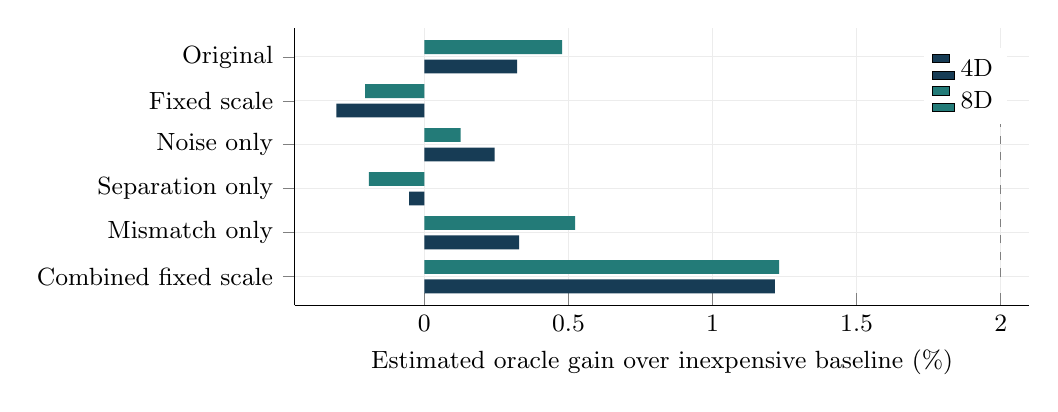
\begin{tikzpicture}
\begin{axis}[xbar,bar width=5pt,width=.90\linewidth,height=5.1cm,xmin=-.45,xmax=2.1,xtick={0,.5,1,1.5,2},ytick=data,symbolic y coords={Combined fixed scale,Mismatch only,Separation only,Noise only,Fixed scale,Original},xlabel={Estimated oracle gain over inexpensive baseline (\%)},grid=major,grid style={gray!15},axis y line*=left,axis x line*=bottom,enlarge y limits=.13,tick label style={font=\small},label style={font=\small},legend style={at={(.97,.93)},anchor=north east,draw=none,font=\small}]
\addplot[fill=ink,draw=none] coordinates {(1.2168,Combined fixed scale)(.3289,Mismatch only)(-.0533,Separation only)(.2434,Noise only)(-.3058,Fixed scale)(.3219,Original)};\addlegendentry{4D}
\addplot[fill=accent,draw=none] coordinates {(1.2308,Combined fixed scale)(.5235,Mismatch only)(-.1931,Separation only)(.1257,Noise only)(-.2055,Fixed scale)(.4784,Original)};\addlegendentry{8D}
\draw[dashed,gray] (axis cs:2,Combined fixed scale)--(axis cs:2,Original);
\end{axis}\end{tikzpicture}
\captionof{figure}{Full controlled heterogeneity study. The dashed line is the prespecified 2\% target. These independently evaluated estimated oracles are not certified upper bounds.}\label{fig:headroom}
\end{center}
\begin{center}\begin{minipage}{\linewidth}\centering\small
\begin{tabular}{@{}lrrr@{}}\toprule
Method & Posterior MSE & Gain vs. cheap (\%) & Gain vs. uniform (\%)\\\midrule
Estimated finite-sample oracle & 37.1642 & 31.67 & 44.05\\
Privileged coverage & 40.2288 & 26.03 & 39.43\\
\textbf{Structured learned coverage} & \textbf{49.9309} & \textbf{8.20} & \textbf{24.83}\\
Matched-feature generic learner & 50.1664 & 7.76 & 24.47\\
Inexpensive rule (floor uncertainty) & 54.3883 & 0.00 & 18.11\\
Learned inverse-$K$ & 64.1326 & -17.92 & 3.44\\
Uniform & 66.4203 & -22.12 & 0.00\\
Direct coverage-coefficient learner & 72.5635 & -33.42 & -9.25\\
Asymptotic oracle & 96.3703 & -77.19 & -45.09\\\bottomrule
\end{tabular}
\captionof{table}{Final UJIIndoorLoc follow-up: 1,111 records, identical draw budgets. Privileged policies use offline exact posterior or risk information; the structured and generic learners do not use the exact test posterior in allocation.}\label{tab:mainwifi}
\end{minipage}\end{center}
\section{Mathematical foundations}
\subsection{Posterior expectations and self-normalized importance sampling}
Let $x_i$ denote observation $i$, $p_i(z)=p_\theta(z\mid x_i)$ the target posterior, and $q_i(z)$ an accessible proposal whose support covers the target. Define the unnormalized weight and marginal likelihood
\begin{equation}
 w_i(z)=\frac{p_\theta(x_i,z)}{q_i(z)},\qquad Z_i=p_\theta(x_i)=\E_{q_i}[w_i(z)].
 \label{eq:weights}
\end{equation}
For a function $h:\R^d\to\R^m$, the posterior quantity of interest is $\mu_i=\E_{p_i}[h(z)]$. Since $p_i/q_i=w_i/Z_i$,
\begin{equation}
 \mu_i=\frac{\E_{q_i}[w_i(z)h(z)]}{\E_{q_i}[w_i(z)]}.
\end{equation}
Given $K_i$ independent proposal draws $z_{ik}\sim q_i$, self-normalized importance sampling (SNIS) estimates this quantity by
\begin{equation}
 \widehat\mu_{i,K_i}=\frac{\sum_{k=1}^{K_i}w_i(z_{ik})h(z_{ik})}{\sum_{k=1}^{K_i}w_i(z_{ik})}
 =\sum_{k=1}^{K_i}\widetilde w_{ik}h(z_{ik}),\qquad
 \widetilde w_{ik}=\frac{w_i(z_{ik})}{\sum_{\ell=1}^{K_i}w_i(z_{i\ell})}.
 \label{eq:snis}
\end{equation}
The ratio estimator is generally biased at finite $K_i$, but is consistent under standard support and integrability assumptions. Throughout the main experiments $h(z)=z$, so $\mu_i$ is the posterior mean vector.
\subsection{Derivation of task-specific asymptotic variance}
For clarity, suppress the observation subscript and let $K$ be the number of draws. Subtracting $\mu$ from Eq.~\eqref{eq:snis} gives the exact identity
\begin{equation}
 \sqrt K(\widehat\mu_K-\mu)=\frac{K^{-1/2}\sum_{k=1}^{K}w(z_k)[h(z_k)-\mu]}{K^{-1}\sum_{k=1}^{K}w(z_k)}.
\end{equation}
The numerator is a sum of centered independent random vectors, because $\E_q[w(h-\mu)]=Z\mu-Z\mu=0$. If its second moment is finite, the multivariate central limit theorem applies. The denominator converges almost surely to $Z>0$ by the law of large numbers. Slutsky's theorem yields
\begin{align}
 \sqrt K(\widehat\mu_K-\mu)&\xrightarrow{d}\N(0,\Gamma_h),\\
 \Gamma_h&=\E_q\!\left[\left(\frac{w(z)}{Z}\right)^2(h(z)-\mu)(h(z)-\mu)^\top\right].
\end{align}
The trace of the covariance defines a scalar task-specific difficulty:
\begin{equation}
 {\tau_{i,h}^{2}=\operatorname{tr}(\Gamma_{i,h})=\E_{q_i}\!\left[\left(\frac{p_i(z)}{q_i(z)}\right)^2\norm{h(z)-\mu_i}^2\right].}
 \label{eq:tau}
\end{equation}
With additional moment conditions sufficient for convergence of second moments, the leading squared-error risk is
\begin{equation}
 \E\norm{\widehat\mu_{i,K_i}-\mu_i}^2\approx\frac{\tau_{i,h}^{2}}{K_i}.
 \label{eq:risk}
\end{equation}
This expression accounts for both proposal--posterior mismatch and the influence of a latent sample on the chosen statistic. A high-weight sample close to the mean has a different contribution from a high-weight sample far from it. For $h(z)=z$ we write $\tau_i=\tau_{i,h}$. Dividing the risk by $d$ gives the per-coordinate MSE used in the experiments; the common factor does not affect the optimal allocation within a dimension.

Equation~\eqref{eq:risk} is an asymptotic approximation, not a finite-budget guarantee. In particular, light-tailed proposals can violate the moment conditions; even when they hold, the online budget of approximately 48 samples per observation may not be in the asymptotic regime.

\subsection{Why ESS is not a task-specific difficulty measure}
The conventional empirical ESS of $K_i$ importance samples is
\begin{equation}
 \widehat{\ESS}_i=\frac{(\sum_k w_{ik})^2}{\sum_k w_{ik}^2}=\frac{1}{\sum_k\widetilde w_{ik}^{\,2}}.
\end{equation}
Writing $r_i=p_i/q_i$, the limiting ESS fraction is $1/\E_{q_i}[r_i^2]$ when the relevant moments exist. It does not include $h(z)$, whereas Eq.~\eqref{eq:tau} contains $\norm{h(z)-\mu_i}^2$. For an explicit counterexample, take exact proposals $q_1=p_1=\N(0,0.01)$ and $q_2=p_2=\N(0,9)$, with $h(z)=z$. Both have constant weights and $\widehat{\ESS}_i=K_i$. Their posterior standard deviations are nevertheless $0.1$ and $3$, so their mean-estimation variances at equal $K_i$ differ by a factor of 900. ESS alone cannot distinguish these tasks.
\subsection{Optimal continuous allocation under a fixed budget}
Let $a_i>0$ denote the relative importance of observation $i$ and let $B$ be the total sample budget. For equal sample-evaluation costs, the idealized objective is
\begin{equation}
 \min_{K_i>0}\ J(K)=\sum_{i=1}^n\frac{a_i\tau_i^2}{K_i},\qquad \sum_{i=1}^n K_i=B.
 \label{eq:opt}
\end{equation}
Assume $\tau_i>0$. The Lagrangian is $\mathcal L=J+\lambda(\sum_i K_i-B)$. The first-order conditions are $-a_i\tau_i^2/K_i^2+\lambda=0$, giving $K_i=\sqrt{a_i}\tau_i/\sqrt\lambda$. The budget condition determines $\sqrt\lambda=\sum_j\sqrt{a_j}\tau_j/B$. Therefore,
\begin{equation}
 {K_i^*=B\frac{\sqrt{a_i}\tau_i}{\sum_j\sqrt{a_j}\tau_j}.}
 \label{eq:optimal}
\end{equation}
Since $\partial^2 J/\partial K_i^2=2a_i\tau_i^2/K_i^3>0$, the stationary point is the unique global minimum of the continuous problem. For equal observation weights, the allocation is proportional to the standard-deviation score $\tau_i$, not to $\tau_i^2$. In that case, Cauchy--Schwarz gives
\begin{equation}
 J^*=\frac{(\sum_i\tau_i)^2}{B}\leq \frac{n}{B}\sum_i\tau_i^2=J_{\mathrm{uniform}}.
\end{equation}
Equality holds when all $\tau_i$ are equal. Thus there is little theoretical room for adaptive allocation if inference difficulties are nearly homogeneous.
\subsection{Sensitivity to learned difficulty errors}
The optimal policy assumes that $\tau_i$ is known. If $s_i>0$ is a prediction, let $b_i=s_i/\sum_j s_j$ and $b_i^*=\tau_i/\sum_j\tau_j$. For equal weights and unrestricted continuous allocation, substituting $K_i=Bb_i$ into Eq.~\eqref{eq:opt} yields
\begin{equation}
 \frac{J(Bb)}{J^*}=\sum_i\frac{(b_i^*)^2}{b_i}=1+\sum_i\frac{(b_i-b_i^*)^2}{b_i}.
 \label{eq:regret}
\end{equation}
The last equality follows from $\sum_i b_i=\sum_i b_i^*=1$. It explains why underallocating a difficult observation can be particularly costly and why ranking accuracy alone may not be sufficient. This identity concerns the asymptotic objective only. Its relationship to finite-sample risk must be tested rather than assumed.


\subsection{Finite-sample risk and allocation sensitivity}
For the main statistic $h(z)=z$, the exact finite-sample objective also has the bias--variance decomposition
\begin{equation}
 R_i(K)=\frac1d\operatorname{tr}\operatorname{Cov}(\widehat\mu_{i,K})+\frac1d\norm{\E\widehat\mu_{i,K}-\mu_i}^2.
\end{equation}
Neither the CLT nor accurate ranking of $\tau_i$ guarantees an accurate risk curve at small $K$. In the asymptotic continuous problem, the relative improvement over uniform is
\begin{equation}
 G_{\rm cont}=1-\frac{(\sum_i\tau_i)^2}{n\sum_i\tau_i^2}=\frac{\operatorname{Var}_i(\tau_i)}{\operatorname{Var}_i(\tau_i)+\E_i[\tau_i]^2}.
\end{equation}
For bounded integer counts, the exact asymptotic optimum assigns each next draw to the largest eligible marginal decrease $\tau_i^2/[K_i(K_i+1)]$, starting at $K_{\min}$. This greedy rule is valid because the marginal decreases are nonincreasing. The same property need not hold for finite-sample risk. For that reason, the proposed allocator solves the discrete optimization directly.

\section{Coverage-aware finite-sample risk}\label{sec:coverage}
\subsection{Probability of missing a task-relevant region}
For each observation, partition the latent space into regions $A_{ij}$, $j=1,\ldots,J$, fixed using the model or development information. Write $\pi_{ij}=p_i(A_{ij})$ and $\rho_{ij}=q_i(A_{ij})$. For independent proposal draws,
\begin{equation}
 \Pr\{z_1,\ldots,z_K\notin A_{ij}\}=(1-\rho_{ij})^K.\label{eq:miss}
\end{equation}
For $0<\pi_{ij}<1$, define $m_{ij}=\E_{p_i}[z\mid A_{ij}]$ and $m_{ij}^{c}=\E_{p_i}[z\mid A_{ij}^c]$. The law of total expectation gives $\mu_i=\pi_{ij}m_{ij}+(1-\pi_{ij})m_{ij}^{c}$. The squared displacement of the posterior mean if the region is excluded is therefore
\begin{equation}
 b_{ij}=\frac1d\norm{\mu_i-m_{ij}^{c}}^2
 =\frac{\pi_{ij}^2}{d}\norm{m_{ij}-m_{ij}^{c}}^2.\label{eq:coveragecoef}
\end{equation}
This combines posterior mass with the sensitivity of the target statistic. A region that is rarely sampled need not matter to the posterior mean if its conditional mean is similar to the complement. Conversely, a region with substantial mass and a distant conditional mean can be consequential even when its proposal mass is small.

\textbf{A motivating exact case.} For a scalar two-point distribution on $\{0,1\}$ with $p(1)=\pi$ and $q(1)=\rho$, let $N\sim\operatorname{Binomial}(K,\rho)$, $w_1=\pi/\rho$, $w_0=(1-\pi)/(1-\rho)$. Its exact finite-sample risk is
\begin{equation}
 R(K)=\sum_{r=0}^K {K\choose r}\rho^r(1-\rho)^{K-r}
 \left(\frac{rw_1}{rw_1+(K-r)w_0}-\pi\right)^2.
\end{equation}
The endpoint terms are $\pi^2(1-\rho)^K$ and $(1-\pi)^2\rho^K$: exactly the contributions of missing either point. Interior terms remain. In general regions, the conditional SNIS estimator on a miss event is random and may be biased even relative to $m_{ij}^{c}$, and several regions can be missed simultaneously. Consequently summing Eq.~\eqref{eq:coveragecoef} times Eq.~\eqref{eq:miss} is not an exact risk decomposition or a bound.
\subsection{Risk surrogate and marginal allocation}
I use the nonnegative surrogate
\begin{equation}
 \boxed{\mathcal R_i(K)=\frac{a_i}{K}+\gamma\sum_{j=1}^{J} b_{ij}(1-\rho_{ij})^K,\qquad a_i\ge0,\ \gamma\ge0.}\label{eq:surrogate}
\end{equation}
The first term represents an inverse-sample component fitted to risk, not necessarily the asymptotic variance. The second is a coverage-sensitive correction. The coefficient $\gamma$ is calibrated on validation data; it does not imply that coverage events are disjoint or that the two terms capture all sources of error. The gain from one extra draw is
\begin{equation}
 \Delta_i(K)=\mathcal R_i(K)-\mathcal R_i(K+1)=\frac{a_i}{K(K+1)}+\gamma\sum_j b_{ij}\rho_{ij}(1-\rho_{ij})^K.\label{eq:marginal}
\end{equation}
Every summand is nonnegative and nonincreasing in $K$. For bounded integer allocations, start at $K_{\min}$ for each observation and repeatedly assign a draw to the eligible observation with the greatest marginal gain. This is optimal for Eq.~\eqref{eq:surrogate}: any feasible allocation selects a prefix of each nonincreasing marginal sequence, and the greedy rule selects the largest feasible remaining marginal. Ties can be broken deterministically. This is an optimization guarantee for the surrogate, not for actual SNIS risk.
\subsection{Structured amortized prediction}
The coefficients in Eq.~\eqref{eq:coveragecoef} are not generally known online. Instead of predicting $b_{ij}$ independently, I estimate normalized masses $\widehat\pi_{ij}$ and conditional moments $\widehat m_{ij}$, reconstructing
\begin{align}
 \widehat\mu_i&=\sum_j\widehat\pi_{ij}\widehat m_{ij},\\
 \widehat m_{ij}^{c}&=\frac{\sum_{\ell\ne j}\widehat\pi_{i\ell}\widehat m_{i\ell}}{\sum_{\ell\ne j}\widehat\pi_{i\ell}},\qquad
 \widehat b_{ij}=\frac1d\norm{\widehat\mu_i-\widehat m_{ij}^{c}}^2.\label{eq:reconstruct}
\end{align}
The implementation guards near-zero complement mass; future work will test the sensitivity of this convention. Proposal probabilities are computed from the fixed proposal and partition, without evaluating the target posterior. The synthetic student predicts region masses and moments directly; the localization student predicts a probability distribution over the surveyed states and aggregates its probabilities and moments by region. The two implementations share the same reconstruction rule.

For each risk-teacher observation, let $\widehat C_i(K)=\sum_j\widehat b_{ij}(1-\rho_{ij})^K$. Given independent replicated risk estimates $\widehat R_i(K)$, fit a nonnegative inverse-$K$ amplitude at each candidate $\gamma$ by weighted least squares:
\begin{equation}
 a_i(\gamma)=\max\left\{\epsilon,\frac{\sum_K \omega_{iK}[\widehat R_i(K)-\gamma\widehat C_i(K)]/K}{\sum_K\omega_{iK}/K^2}\right\}.
\end{equation}
The weights in the implementation are inverse squared risk with a positive floor. A histogram gradient-boosting regressor predicts $\log a_i$ from accessible features and the student's outputs. The generic risk predictors receive the same student-derived features, including the reconstructed coverage summaries, so the comparison tests the explicit risk structure rather than merely access to better inputs.
\subsection{Reliability and baseline-aware optimization}
Let $K^0$ be a cheap allocation selected on validation data. The completed structured study minimizes
\begin{equation}
 \min_{\mathbf K}\sum_i\left[\widehat{\mathcal R}_i(K_i)+\lambda s_{\mathrm{batch}}|K_i-K_i^0|\right],\quad \sum_i K_i=B,\label{eq:penalty}
\end{equation}
with the original integer bounds and $s_{\mathrm{batch}}$ equal to the median predicted risk at $K=48$ divided by 48 (with a floor). Validation considers $\gamma\in\{0.1,0.25,0.5,1,2\}$, $\lambda\in\{0,0.25,1,4\}$ and full fallback. The penalty is separable and discretely convex for the coverage surrogate, so its net marginal gains are nonincreasing as well. The implemented optimizer uses exact dynamic programming, which also handles generic nonconvex risk curves: $D_j(b)=\min_k[D_{j-1}(b-k)+\widehat{\mathcal R}_j(k)+\lambda s_{\mathrm{batch}}|k-K_j^0|]$, with infeasible states infinite. Backtracking yields feasible counts. Its worst-case time is $O(nB(K_{\max}-K_{\min}+1))$; greedy optimization of the structured surrogate is a prospective efficiency improvement.

In the final real-data study, validation selected $\gamma=1$ and $\lambda=0$. The resulting method reduced average error, but harmed 14 of 35 batches relative to the cheap rule. The penalty therefore did not establish a reliability benefit. A future reliability policy must distinguish likely gains from harmful reallocations, not merely improve average validation MSE.
\section{Proposed research and hypotheses}
The preliminary studies establish a concrete problem and a candidate solution. They do not establish broad superiority over generic risk prediction or a practical speed advantage. The following aims are prospective.
\subsection{Aim 1 (H1): characterize when coverage is informative}
\textbf{Hypothesis.} Under finite budgets, task-sensitive posterior coverage provides useful information about marginal risk reductions beyond simple scale features in regimes with meaningful allocation headroom.

Define the true finite-sample headroom for a fixed baseline $\mathbf K^0$ by
\begin{equation}
 G_{\mathrm{finite}}=1-\frac{\min_{\mathbf K\ \mathrm{feasible}}\sum_i R_i(K_i)}{\sum_i R_i(K_i^0)}.
\end{equation}
It is nonnegative when the denominator is positive. An independently evaluated estimated oracle is an empirical benchmark, not a certified upper bound on possible improvement. I will study how coverage, proposal mismatch, region geometry and sampling budgets affect the difference between this benchmark and cheap allocation. The completed synthetic study indicates that heterogeneity alone does not guarantee useful gains. I will compare controlled partitions, matched-feature coverage ablations, power-law and flexible curves, and Monte Carlo estimates with independent evaluation banks of increasing precision. In particular, I will investigate whether the coverage surrogate captures the actual marginal risk rather than simply improving calibration at one sample count.

If the estimated oracle does not exceed the cheap baseline by a practically meaningful amount, I will characterize the allocation limits in that regime instead of training a more complex predictor. This constitutes an independent research outcome. For fitted risk curves $\widetilde R_i$ satisfying $\sup_k|\widetilde R_i(k)-R_i(k)|\le\epsilon_i$, an exact minimizer of the fitted objective obeys $\sum_i R_i(\widetilde K_i)-\sum_i R_i(K_i^*)\le 2\sum_i\epsilon_i$ by adding and subtracting both fitted objectives and using fitted optimality. This elementary bound motivates calibration and uncertainty analysis; it is not a claim that such error bounds have been established empirically.
\subsection{Aim 2 (H2): generalize structured coverage prediction}
\textbf{Hypothesis.} Reconstructing statistic sensitivity from coherent posterior-region predictions can achieve useful allocation gains on previously unexamined inference tasks at matched budgets, while using only accessible online information.

I will freeze the current formulation, evaluate on untouched real-data cohorts or datasets with independent buildings/devices, and compare against validation-selected cheap rules and generic learners receiving the same features. I will test whether errors in predicted masses and conditional moments jointly affect marginal utility. In the completed final study, replacing predicted masses with exact masses while keeping the learned amplitude fixed actually increased MSE, and replacing moments alone did not improve it significantly. These substitutions are not refitted models and do not establish which component is intrinsically deficient. I will examine jointly calibrated amplitudes and region predictions, alternative partitions chosen only on development data, and the effect of teacher precision. Where reliable posterior labels are expensive, I will test replicate-based variance labels plus bias estimates against tractable references before using them as surrogates.
\subsection{Aim 3 (H3): reliable and computationally worthwhile allocation}
\textbf{Hypothesis.} Validation-calibrated reliability policies can reduce the frequency and severity of harmful allocations while preserving most of the positive average gain, in settings where allocation is computationally justified.

I will compare the penalty in Eq.~\eqref{eq:penalty} with batch-specific shrinkage $K_i(\alpha)=(1-\alpha)K_i^0+\alpha K_i^L$ followed by exact-budget largest-remainder rounding. Reliability indicators will include disagreement across student fits or teacher banks, validation risk calibration and accessible proposal summaries. These indicators must not rely on exact test posterior information. If positive gain is not reliable, the policy may abstain and use the baseline. I will evaluate mean risk, harmful-batch fraction and worst-decile relative loss, including uncertainty over independent batches.

A separate cost comparison will include direct enumeration, direct amortized posterior prediction, numerical integration when appropriate, uniform SNIS and cheap allocation. In particular, the final localization experiment took 77.14 ms for structured allocation versus 1.82 ms for exact enumeration in a single-batch CPU benchmark. The 8.20\% gain is an equal-draw-budget result, not an end-to-end speedup. I will study larger state spaces or continuous latent models with expensive likelihoods, measure actual target-evaluation costs and use the greedy surrogate optimizer where applicable. If exact or direct inference remains preferable, I will report the boundary of applicability rather than claim an advantage.
\subsection{Testbeds}
Use the completed Gaussian mixtures as controls and the fitted UJIIndoorLoc pipeline as a reproducible exploratory benchmark. For independent validation, identify another real-data cohort or dataset before evaluation; if no independent cohort is available, limit claims to synthetic confirmation and exploratory real-data evidence. A two-dimensional nonlinear model $z\sim\N(0,I_2)$, $x=g(z)+\epsilon$, $g(z)=(z_1^2+0.5z_2,\sin z_1+z_2)^\top$, $\epsilon\sim\N(0,\sigma^2I_2)$, permits grid-refined reference means. VAE transfer will use independent fitted-model seeds and HMC references with rank-normalized $\widehat R<1.01$, effective sample size and integration checks. These diagnostics are necessary, not proof of reference accuracy.
\section{Evaluation protocol and decision criteria}
Freeze data splits, partition construction, teacher budget, candidate policies, metrics and thresholds on development data. For synthetic experiments, use independent batches as the unit of inference. For new real data, use appropriate independent deployment groups rather than treating repeated Monte Carlo trials as independent environments. Report paired effect sizes and intervals, multiplicity-adjusted primary comparisons, reference coverage and model-seed sensitivity. The reused UJIIndoorLoc records will not be used to confirm generalization. The following prospective targets retain the original 2\% feasibility criterion and distinguish predictive improvement from mechanism and reliability.
\begin{center}\begin{minipage}{\linewidth}\centering\small
\begin{tabularx}{\linewidth}{@{}p{.85in}Y@{}}\toprule
Aim & Proposed criterion\\\midrule
Feasibility & At least 2\% independently evaluated estimated oracle gain over the validation-selected cheap rule, with paired interval excluding zero. Audit sensitivity to oracle-bank size.\\
H1 & Positive coverage ablation at matched information, and useful marginal-risk calibration in prespecified regimes with stable headroom.\\
H2 & At least 2\% reduction over the cheap baseline, paired 95\% interval excluding zero; capture at least 25\% of stable estimated headroom and test superiority over the strongest matched-feature generic model separately.\\
H3 & Reduce both harmed-batch frequency and worst-decile loss while retaining at least 75\% of positive mean gain. If no positive gain exists, evaluate fallback alone.\\
Cost & Report time-to-matched-error including feature extraction, posterior student, optimizer and sampling; compare with direct inference.\\\bottomrule
\end{tabularx}\captionof{table}{Proposed independent evaluation criteria. A missed criterion remains a reportable outcome.}\end{minipage}\end{center}
For an intended reuse volume $N$, report $T_{\rm build}/N+T_{\rm online}$ against the total cost of competing policies. Include teacher simulations, posterior-label computation, model fitting, calibration, and memory. The original 409,600-draw teacher would require roughly 720 batches to recover its cost by evaluation count under the illustrative 10\% gain and local $K^{-0.8}$ scaling; this does not establish break-even against cheap allocation or the new structured method. The new method needs its own measured cost accounting.
\section{Plan, risks and contingencies}
\begin{center}\begin{minipage}{\linewidth}\centering\small
\begin{tabularx}{\linewidth}{@{}p{.77in}YY@{}}\toprule
Months & Work & Deliverable\\\midrule
1--3 & Literature comparison, coverage mechanism and risk-estimation audits & Characterization of headroom and surrogate limits\\
4--9 & Freeze candidate models; independent data and controlled validation & H1/H2 results and manuscript draft\\
10--14 & Reliability calibration, tail loss and cost-aware evaluation & H3 result and measured efficiency limits\\
15--18 & Larger or continuous inference tasks; validated reference transfer & Consolidated manuscript and reproducible evaluation\\\bottomrule
\end{tabularx}\captionof{table}{Eighteen-month research plan building on completed studies.}\end{minipage}\end{center}
\begin{center}\begin{minipage}{\linewidth}\centering\small
\begin{tabularx}{\linewidth}{@{}YY@{}}\toprule
Risk & Response\\\midrule
Little additional headroom & Characterize regimes where simple allocation suffices; avoid unnecessary learning.\\
Structured predictor matches but does not beat generic learning & Report comparable performance, test interpretability and computational cost; do not claim predictive superiority.\\
Coverage terms double-count missed regions or poorly predict marginal gains & Audit region partitions and surrogate error; restrict claims to supported regimes.\\
Reference estimates or transfer unreliable & Report coverage, use independent references and limit generalization claims.\\
Harm persists or direct inference is faster & Use validated fallback; quantify limits and compare in expensive-likelihood settings.\\\bottomrule
\end{tabularx}\captionof{table}{Main risks and contingency plans.}\end{minipage}\end{center}
\section{Related work and expected contribution}
The continuous allocation rule follows Neyman allocation \cite{neyman1934} applied to SNIS asymptotic variance \cite{owen2013}. Sample-size requirements for importance sampling \cite{chatterjee2018} motivate studying proposal--target mismatch at finite budgets. ESS alternatives \cite{martino2017} describe weight quality; adaptive importance sampling \cite{bugallo2017} primarily improves proposals, whereas this work keeps them fixed. Amortized inference \cite{gershman2014,cremer2018} learns reusable inference procedures, while importance-weighted variational objectives \cite{burda2016,rainforth2018,tucker2019} address training. Simulation-based inference \cite{cranmer2020} provides a broader motivation for repeated inference. The proposed contribution is not SNIS itself, the law of total expectation, or the integer optimizer. It is a task-sensitive coverage risk surrogate, coherent amortized reconstruction of its coefficients, and an investigation of when that structure can improve fixed-budget allocation. The positive preliminary learned result motivates independent tests, but the available literature comparison is not a comprehensive novelty review. The relationship to existing finite-sample, rare-region and allocation methods must be established before claiming originality.
\clearpage
\appendix
\section{Completed-study protocols and detailed results}\label{app:protocol}
\subsection{Original learning-based allocation method}
\subsubsection{Offline teacher estimates}
The quantity in Eq.~\eqref{eq:tau} is unknown for a new observation. A pilot can estimate difficulty at test time, but its draws consume part of the inference budget. The original method estimates difficulty on development observations and trains a supervised regressor; Section~\ref{sec:baselines} tests the cost of a pilot explicitly. For each development observation, draw $M=\dev$ samples from its proposal and calculate the normalized weights and teacher posterior mean $\widetilde\mu_i=\sum_k\widetilde w_{ik}z_{ik}$. Replacing the expectation and normalizer in Eq.~\eqref{eq:tau} by their sample counterparts gives
\begin{equation}
 \widehat\tau_i^2=M\sum_{k=1}^{M}\widetilde w_{ik}^{\,2}\norm{z_{ik}-\widetilde\mu_i}^2.
 \label{eq:teacher}
\end{equation}
The synthetic implementation uses $s_i^{\task}=\sqrt{\max(\widehat\tau_i^2,10^{-5})+0.02}$ and $s_i^{\mathrm{ESS}}=\sqrt{\max(M/\widehat{\ESS}_i-1,0)+0.05}$. These are finite-sample proxies, not exact labels; the positive offsets stabilize the allocation. The later VAE code uses offsets outside the square roots. The same synthetic teacher convention is retained in the new comparisons.
\subsubsection{Amortized prediction of estimation difficulty}
Let $F(x_i)$ be inexpensive observation and proposal features. I fit a histogram gradient-boosting regressor $f$ to log teacher scores, using a squared-error objective with regularization. The predicted positive score is $s_i=\exp(f(F(x_i)))$. Both learned allocators use the same regressor family: 130 boosting iterations, at most 10 leaves per tree, learning rate 0.1, at least 20 samples per leaf and $L_2$ regularization 2.0. The models differ principally in the teacher target. The task predictor estimates sampling difficulty, not the posterior mean itself. Predictions are fixed before final testing.


\subsubsection{Integer allocation and online inference}
In the implementation, $K_{\min}=4$ and $K_{\max}=120$. Reserve $K_{\min}$ draws per observation, and distribute the remaining budget according to the predicted scores. The continuous intermediate counts are
\begin{equation}
 k_i=K_{\min}+\min\{K_{\max}-K_{\min},\ c\,s_i\},\qquad\sum_i k_i=B,
\end{equation}
where $c$ is found by bisection. Floor the extra counts and assign residual draws in descending fractional-remainder order to eligible observations. This produces feasible integer counts and exactly preserves the budget. It is a stabilized, capped proportional-extras heuristic inspired by Eq.~\eqref{eq:optimal}, not the exact bounded optimum. Finally, apply Eq.~\eqref{eq:snis} using the allocated samples. Inference requires feature extraction and regression, but no online teacher draws. Offline costs are accounted for separately from online sampling costs.


\subsection{Analytically tractable Gaussian mixtures}
\subsubsection{Model and evaluation design}
The synthetic model uses a two-component prior and a Gaussian observation model with context $c$ controlling the noise scale:
\begin{equation}
 p(z)=\sum_{j=1}^2\pi_j\N(z;m_j,I_d),\qquad p(x\mid z,c)=\N(x;z,\sigma_c^2 I_d),\quad d\in\{4,8\}.
\end{equation}
Completing the square gives a Gaussian-mixture posterior. Component $j$ has conditional mean $m_j'(x,c)=(x+\sigma_c^2m_j)/(1+\sigma_c^2)$ and covariance $\sigma_c^2 I_d/(1+\sigma_c^2)$. Its posterior weight is
\begin{equation}
 \gamma_j(x,c)=\frac{\pi_j\N(x;m_j,(1+\sigma_c^2)I_d)}{\sum_{\ell=1}^2\pi_\ell\N(x;m_\ell,(1+\sigma_c^2)I_d)}.
\end{equation}
Hence the exact posterior mean is $\mu(x,c)=\sum_j\gamma_j m_j'$. The marginal likelihood is
\[Z(x,c)=\sum_j\pi_j\N(x;m_j,(1+\sigma_c^2)I_d).\] The proposal is a single Gaussian; the exact posterior is not supplied to the learned predictor. The regressors receive $x$, $x^{\odot 2}$, $\norm{x}$, the proposal mean norm, proposal standard deviation, observation-noise standard deviation, and context index ($2d+5$ features).

\begin{center}
\small
\begin{tabularx}{\linewidth}{@{}lY@{}}
\toprule
Development & 800 observations per dimension; development seed 742; $\dev\in\{512,1024,2048\}$.\\
Pilot & Four held-out datasets (seeds 13, 37, 71, 101), 16 paired Monte Carlo trials each.\\
Confirmation & 25 new datasets per dimension (seeds 1001--1025); unchanged predictors; 16 trials each.\\
Online budget & 84 observations per dataset; 48 samples on average; $B=4032$.\\
Methods & Uniform, amortized ESS-derived allocation and task-aware allocation.\\
\bottomrule
\end{tabularx}
\captionof{table}{Synthetic experimental protocol. The 512-sample primary comparison was chosen after the pilot and checked on new datasets.}
\end{center}
The primary metric is $\MSE=\frac{1}{nd}\sum_i\norm{\widehat\mu_i-\mu_i}^2$; the secondary metric is $\frac1n\sum_i|\log\widehat Z_i-\log Z_i|$, where $\widehat Z_i=K_i^{-1}\sum_k w_{ik}$. For inference, average the paired trial differences within each dataset and then use dataset-level differences to calculate Student-$t$ intervals and sign-flip tests. Individual observations and Monte Carlo repetitions are not treated as independent datasets.
\subsubsection{Pilot and independent confirmation}
The four-dataset pilot found reductions of 11.65\% (4D) and 9.34\% (8D) at $\dev=512$. The exact two-sided sign-flip test had $p=0.125$ in both dimensions; the pilot was therefore not conclusive. The confirmation used the frozen predictors on new datasets. Its results are shown in Table~\ref{tab:synth}.
\begin{center}
\small
\begin{tabular}{@{}rr rrr rr@{}}
\toprule
$d$ & $\dev$ & Uniform & ESS-based & Task-aware & vs. uniform & vs. ESS\\
\midrule
4&512&0.087952&0.090669&0.079014&10.16\%&12.85\%\\
4&1024&0.087952&0.092471&0.079244&9.90\%&14.30\%\\
4&2048&0.087952&0.092113&0.079817&9.25\%&13.35\%\\
8&512&0.079915&0.081337&0.072789&8.92\%&10.51\%\\
8&1024&0.079915&0.082272&0.073244&8.35\%&10.97\%\\
8&2048&0.079915&0.082428&0.073349&8.22\%&11.01\%\\
\bottomrule
\end{tabular}
\captionof{table}{Per-coordinate posterior-mean MSE on the 25 confirmation datasets per dimension. The last two columns report relative error reductions.}\label{tab:synth}
\end{center}



\subsection{Matched-budget baseline audit}\label{sec:baselines}
\subsubsection{Design and comparators}
The original 512-draw predictors were reconstructed from the same development seed (742), model, features and teacher code. I retained the original 25 confirmation datasets (1001--1025) and generated 25 fresh datasets (2001--2025) per dimension, with 84 observations and 16 paired trials per dataset. The original proposal is $q_i=\N(b_i,u_i I_d)$, where
\begin{equation}
 b_i=\frac{0.88x_i}{1+\sigma_{c_i}^2},\quad
 u_i=\frac{\sigma_{c_i}^2}{1+\sigma_{c_i}^2}\,a_{c_i}^{2},\quad
 (\sigma_c)=(0.45,1,2.1),\ (a_c)=(1,1.1,1.25).
\end{equation}
The mixture has weights $(0.55,0.45)$ and prior means $\pm 2.25 e_1$. Every method consumes exactly $B=4032$ density evaluations per trial and at most 120 per observation. Fixed-score policies share the same sample bank. Pilot policies use a separate eight-draw pilot bank and matched fresh draws; reuse requires $K_i\geq8$, and discard leaves 4--112 final draws per observation. The offline learned predictors consume 409,600 teacher evaluations per dimension, excluding model fitting.

\begin{center}\begin{minipage}{\linewidth}\centering\small
\begin{tabularx}{\linewidth}{@{}lY@{}}
\toprule
Method & Allocation score or rule\\
\midrule
Uniform & Equal counts, 48 draws per observation.\\
Amortized ESS; Learned task & Original fitted predictors, using weight variability or task-specific variance.\\
Context noise; Proposal width & $\sigma_c$ or $\sqrt{u_i}$; no training or pilot required.\\
Posterior-scale oracle & $\sqrt{\operatorname{tr}\operatorname{Cov}_{p_i}(z)}$, available analytically only here.\\
Variance oracles & Exact $\tau_i$ with original capped-extras rule or exact integer optimum.\\
Pilot8Fresh; Pilot8Reuse & Estimate the original teacher score from eight pilot draws. Discard or reuse these draws, counting them toward $B$.\\
Uniform pilot controls & Same pilot discard (40 fresh draws) or reuse (48 total draws) without adaptive allocation.\\
\bottomrule
\end{tabularx}
\captionof{table}{Baseline policies. Only oracle methods use analytic posterior information for allocation.}
\end{minipage}\end{center}
\subsubsection{Results on original and fresh datasets}
\begin{center}\begin{minipage}{\linewidth}\centering\small
\begin{tabular}{@{}lrrrr@{}}
\toprule
&\multicolumn{2}{c}{Original confirmation}&\multicolumn{2}{c}{Fresh follow-up}\\
\cmidrule(lr){2-3}\cmidrule(l){4-5}
Method & 4D & 8D & 4D & 8D\\
\midrule
Context noise &11.89&10.30&\textbf{11.90}&\textbf{10.25}\\
Proposal width &11.28&10.24&11.45&10.18\\
Posterior-scale oracle &10.86&9.51&10.96&9.43\\
Learned task &10.16&8.92&10.45&8.88\\
Variance oracle (integer optimum)&6.84&5.59&6.50&5.48\\
Variance oracle (original rule)&6.58&5.47&6.34&5.31\\
Pilot8Reuse&6.09&2.60&5.10&2.85\\
Uniform&0&0&0&0\\
Uniform48ReusePilot&0.71&$-0.45$&$-0.94$&$-0.39$\\
Amortized ESS&$-3.09$&$-1.78$&$-3.99$&$-2.01$\\
Pilot8Fresh&$-8.20$&$-9.19$&$-8.95$&$-9.82$\\
Uniform40DiscardPilot&$-14.46$&$-14.13$&$-15.00$&$-14.48$\\
\bottomrule
\end{tabular}
\captionof{table}{Percentage reduction in posterior-mean MSE relative to uniform, with 25 datasets per dimension and cohort. Positive values favor the indicated method. The original learned results are reproduced, not counted as independent new evidence.}\label{tab:baselines}
\end{minipage}\end{center}

\begin{center}\begin{minipage}{\linewidth}\centering\small
\begin{tabular}{@{}llrrr@{}}
\toprule
$d$ & Paired contrast (learned minus baseline) & Difference & 95\% $t$ interval & Learned lower\\
\midrule
4 & Context noise & $+0.001242$ & $[0.000668,0.001817]$ &5/25\\
4 & Proposal width & $+0.000852$ & $[0.000538,0.001166]$ &3/25\\
8 & Context noise & $+0.001073$ & $[0.000653,0.001493]$ &4/25\\
8 & Proposal width & $+0.001018$ & $[0.000748,0.001289]$ &1/25\\
\bottomrule
\end{tabular}
\captionof{table}{Fresh datasets: paired differences in per-coordinate MSE. All four intervals exclude zero; positive differences favor the cheap rule. Monte Carlo sign-flip $p$-values range from 0.000020 to 0.000160.}\label{tab:cheap}
\end{minipage}\end{center}
The original gain over uniform is reproducible: at $\dev=512$, the original paired 95\% intervals were $[-0.009609,-0.008266]$ (4D) and $[-0.007610,-0.006643]$ (8D). The learned method beat uniform and amortized ESS on all 25 original datasets at each teacher budget, but the learned component has no demonstrated advantage over the accessible heuristics. These results are conditional on the fitted predictors. Within-component posterior scale is $\sigma_c/\sqrt{1+\sigma_c^2}$, whose derivative is $(1+\sigma_c^2)^{-3/2}>0$. Context noise and proposal width are thus informative by construction; the full posterior also has between-component variance. The results are consistent with learning largely scale-related information, but do not identify the regressor's internal feature dependence.

The eight-draw pilot consumes 672 of 4032 evaluations. Discarding these draws leaves 3360 fresh draws; the adaptive fresh pilot nevertheless beats its uniform-40 control. Reusing pilot draws improves over uniform by 5.10\% and 2.85\% in the fresh cohort and beats its matched reuse control. Reuse changes the sampling rule adaptively and may alter finite-sample bias. The learned allocator beats both pilot variants, but neither amortization nor pilot sampling is universally preferable. This comparison tests sample counts, not total runtime or amortization break-even.

\subsection{Analytical variance and oracle headroom}
For the synthetic model, the exact posterior has two Gaussian components with means $m_j'$ and common covariance $vI_d$, where $v=\sigma_c^2/(1+\sigma_c^2)$. To evaluate Eq.~\eqref{eq:tau} without noisy importance weights, expand $p(z)^2/q(z)$ into four Gaussian-product terms. Center coordinates at the proposal mean $b$, let $y=z-b$, $a_j=m_j'-b$, $t=\mu-b$, and $q=\N(b,u I_d)$. For each pair $(j,k)$, define
\begin{align}
 A&=2/v-1/u,\quad h_{jk}=(a_j+a_k)/v,\quad \ell_{jk}=h_{jk}/A,\\
 C_{jk}&=\frac{(2\pi u)^{d/2}}{(2\pi v)^d}\left(\frac{2\pi}{A}\right)^{d/2}
 \exp\!\left[-\frac12\left(\frac{\norm{a_j}^2+\norm{a_k}^2}{v}-\frac{\norm{h_{jk}}^2}{A}\right)\right].
\end{align}
Completing the square in $y$ gives a Gaussian with mean $\ell_{jk}$ and covariance $A^{-1}I_d$, multiplied by $C_{jk}$. Consequently,
\begin{equation}
 {\tau_i^2=\sum_{j,k}\gamma_j\gamma_k C_{jk}\left[d/A+\norm{\ell_{jk}-t}^{2}\right].}
\end{equation}
The integral is finite if $A>0$. Here $u=a_c^2v\geq v>0$, so this condition holds. In the exact-proposal case $q=p$, the score reduces to the trace of the posterior covariance. The notebook uses log-space accumulation and checks positivity and finiteness.

For equal observation weights, define the unrestricted continuous headroom
\begin{equation}
 G_{\rm cont}=1-\frac{J^*}{J_U}=1-\frac{(\sum_i\tau_i)^2}{n\sum_i\tau_i^2}
 =\frac{\operatorname{Var}_i(\tau_i)}{\operatorname{Var}_i(\tau_i)+\E_i[\tau_i]^2}.
\end{equation}
For the bounded integer problem, start at $K_i=4$ and successively assign one draw to the eligible observation with largest $\tau_i^2/[K_i(K_i+1)]$, stopping at the exact budget. This is optimal for the separable asymptotic objective because each marginal gain decreases with $K_i$. Let $J_O$ be this bounded optimum and $J_L$ the learned allocation's asymptotic risk. The captured fraction is $(J_U-J_L)/(J_U-J_O)$, using the same theoretical risk in all terms. The empirical oracle is evaluated separately with independent online draws, using the analytic posterior mean.
\begin{center}\begin{minipage}{\linewidth}\centering\small
\begin{tabular}{@{}lrrrr@{}}
\toprule
&\multicolumn{2}{c}{Original confirmation}&\multicolumn{2}{c}{Fresh follow-up}\\
\cmidrule(lr){2-3}\cmidrule(l){4-5}
Quantity (\%)&4D&8D&4D&8D\\
\midrule
Continuous asymptotic headroom&8.39&8.48&9.09&9.58\\
Bounded asymptotic headroom&8.37&8.45&9.06&9.46\\
Learned asymptotic headroom captured&37.11&28.55&32.73&25.29\\
Measured gain, bounded variance oracle&6.84&5.59&6.50&5.48\\
Measured gain, learned task&10.16&8.92&10.45&8.88\\
Measured learned/oracle gain ratio&148.61&159.53&160.84&162.10\\
\bottomrule
\end{tabular}
\captionof{table}{Oracle summary. Headroom and capture are ratios of cohort-mean asymptotic risks; the last three rows use measured finite-sample MSE. A ratio above 100\% in the last row does not violate the theoretical optimum: that oracle minimizes a different objective.}\label{tab:oracle}
\end{minipage}\end{center}

\subsection{Additional baseline and risk-calibration figures}
\begin{center}
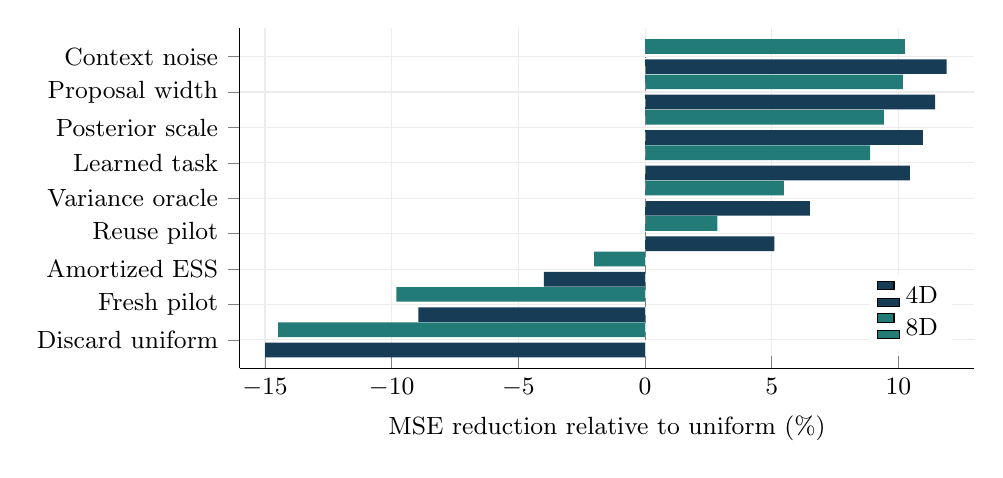
\begin{tikzpicture}
\begin{axis}[xbar,bar width=5.3pt,width=0.90\linewidth,height=5.9cm,xmin=-16,xmax=13,xtick={-15,-10,-5,0,5,10},ytick=data,symbolic y coords={Discard uniform,Fresh pilot,Amortized ESS,Reuse pilot,Variance oracle,Learned task,Posterior scale,Proposal width,Context noise},xlabel={MSE reduction relative to uniform (\%)},grid=major,grid style={gray!15},axis y line*=left,axis x line*=bottom,enlarge y limits=.10,tick label style={font=\small},label style={font=\small},legend style={at={(0.97,0.05)},anchor=south east,draw=none,font=\small}]
\addplot[fill=ink,draw=none] coordinates {(-15.00,Discard uniform)(-8.95,Fresh pilot)(-3.99,Amortized ESS)(5.10,Reuse pilot)(6.50,Variance oracle)(10.45,Learned task)(10.96,Posterior scale)(11.45,Proposal width)(11.90,Context noise)};\addlegendentry{4D}
\addplot[fill=accent,draw=none] coordinates {(-14.48,Discard uniform)(-9.82,Fresh pilot)(-2.01,Amortized ESS)(2.85,Reuse pilot)(5.48,Variance oracle)(8.88,Learned task)(9.43,Posterior scale)(10.18,Proposal width)(10.25,Context noise)};\addlegendentry{8D}
\draw[gray,dashed] (axis cs:0,Discard uniform)--(axis cs:0,Context noise);
\end{axis}
\end{tikzpicture}
\captionof{figure}{Fresh-cohort results from the reported full-run summary (Table~\ref{tab:baselines}). The variance oracle is the exact bounded integer asymptotic optimum. Uniform is the zero reference.}
\end{center}

\subsection{Finite-sample risk audit}
For each dimension, 12 observations per fresh dataset were randomly selected before risk inspection (300 observations from 25 datasets). For each observation I ran 1,024 independent SNIS repetitions, recording every prefix size $K=4,\ldots,120$ using the exact posterior mean. The nested prefixes share randomness across $K$ but each repetition is independent. Let
\begin{equation}
 R_i(K)=\frac1d\E\norm{\widehat\mu_{i,K}-\mu_i}^{2},\qquad
 \widehat R_i(K)=\frac{1}{1024d}\sum_{r=1}^{1024}\norm{\widehat\mu^{(r)}_{i,K}-\mu_i}^{2}.
\end{equation}
The theoretical prediction is $A_i(K)=\tau_i^2/(dK)$, and the calibration ratio is $C_i(K)=\widehat R_i(K)/A_i(K)$. Figures~\ref{fig:risk} and~\ref{fig:cal} use the nine reported sample counts from the full-run summary; the underlying experiment evaluated all 117 counts.
\begin{center}\begin{minipage}{\linewidth}
\centering
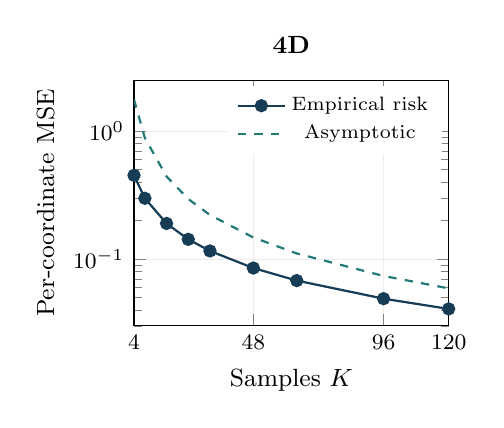
\begin{tikzpicture}
\begin{axis}[width=0.46\linewidth,height=4.7cm,xmin=4,xmax=120,xtick={4,48,96,120},xlabel={Samples $K$},grid=major,grid style={gray!15},tick label style={font=\footnotesize},label style={font=\small},title style={font=\small\bfseries},legend style={draw=none,font=\scriptsize,at={(0.98,0.98)},anchor=north east},title={4D},ymode=log,ymin=0.03,ymax=2.5,ylabel={Per-coordinate MSE}]
\addplot[ink,thick,mark=*] coordinates {(4,0.45178) (8,0.29878) (16,0.18995) (24,0.14268) (32,0.11575) (48,0.08507) (64,0.06787) (96,0.04900) (120,0.04075)};\addlegendentry{Empirical risk}
\addplot[accent,dashed,thick] coordinates {(4,1.77039) (8,0.88520) (16,0.44260) (24,0.29507) (32,0.22130) (48,0.14753) (64,0.11065) (96,0.07377) (120,0.05901)};\addlegendentry{Asymptotic}
\end{axis}
\end{tikzpicture}\hfill
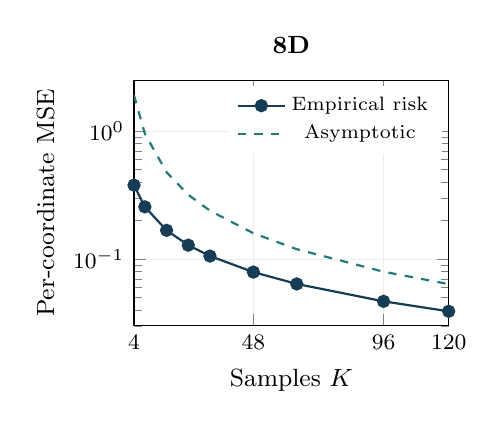
\begin{tikzpicture}
\begin{axis}[width=0.46\linewidth,height=4.7cm,xmin=4,xmax=120,xtick={4,48,96,120},xlabel={Samples $K$},grid=major,grid style={gray!15},tick label style={font=\footnotesize},label style={font=\small},title style={font=\small\bfseries},legend style={draw=none,font=\scriptsize,at={(0.98,0.98)},anchor=north east},title={8D},ymode=log,ymin=0.03,ymax=2.5,ylabel={Per-coordinate MSE}]
\addplot[ink,thick,mark=*] coordinates {(4,0.37856) (8,0.25606) (16,0.16781) (24,0.12846) (32,0.10562) (48,0.07912) (64,0.06388) (96,0.04670) (120,0.03903)};\addlegendentry{Empirical risk}
\addplot[accent,dashed,thick] coordinates {(4,1.91161) (8,0.95581) (16,0.47790) (24,0.31860) (32,0.23895) (48,0.15930) (64,0.11948) (96,0.07965) (120,0.06372)};\addlegendentry{Asymptotic}
\end{axis}
\end{tikzpicture}
\captionof{figure}{Mean empirical SNIS risk and exact asymptotic prediction, on randomly selected fresh observations. Both dimensions use the same logarithmic vertical scale. The theoretical curve substantially overestimates measured risk in the tested range.}\label{fig:risk}
\end{minipage}\end{center}
\begin{center}\begin{minipage}{\linewidth}\centering\small
\begin{tabular}{@{}rr rrr rr@{}}
\toprule
$d$ & $K$ & Empirical MSE & Asymptotic MSE & Ratio of means & Median ratio & Spearman $\rho$\\
\midrule
4&4&0.45178&1.77039&0.25518&0.27212&0.78602\\
4&48&0.08507&0.14753&0.57660&0.61984&0.84202\\
4&120&0.04075&0.05901&0.69053&0.74354&0.84938\\
8&4&0.37856&1.91161&0.19803&0.24768&0.78962\\
8&48&0.07912&0.15930&0.49664&0.60640&0.78939\\
8&120&0.03903&0.06372&0.61248&0.74524&0.80727\\
\bottomrule
\end{tabular}
\captionof{table}{Selected finite-sample diagnostics. Ratio of means is distinct from median per-observation calibration; $\rho$ measures the association between empirical risk and $\tau_i^2$.}\label{tab:risk}
\end{minipage}\end{center}
At $K=48$, the asymptotic prediction is about 1.73 times the measured mean risk in 4D and 2.01 times in 8D. Only 34 of 300 and 1 of 300 observations, respectively, have $0.8\leq C_i(48)\leq1.2$. Even at 120 draws, only 43\% and 35\% meet this criterion. These are empirical Monte Carlo risk estimates, not exact finite-sample integrals; their dispersion is assessed across observations rather than treated as independent confidence intervals.

\subsection{Calibration and task dependence}
\begin{center}\begin{minipage}{\linewidth}
\centering
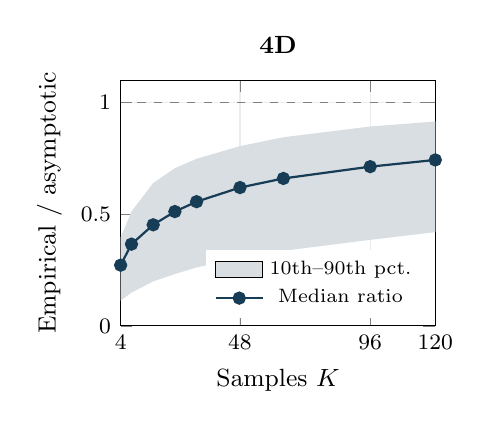
\begin{tikzpicture}
\begin{axis}[width=0.46\linewidth,height=4.7cm,xmin=4,xmax=120,xtick={4,48,96,120},xlabel={Samples $K$},grid=major,grid style={gray!15},tick label style={font=\footnotesize},label style={font=\small},title style={font=\small\bfseries},legend style={draw=none,font=\scriptsize,at={(0.98,0.98)},anchor=north east},title={4D},ymin=0,ymax=1.1,ylabel={Empirical / asymptotic},legend style={draw=none,font=\scriptsize,at={(0.97,0.03)},anchor=south east}]
\addplot[name path=lower,draw=none,forget plot] coordinates {(4,0.11345) (8,0.14925) (16,0.19929) (24,0.23244) (32,0.26197) (48,0.30330) (64,0.33644) (96,0.38553) (120,0.42005)};
\addplot[name path=upper,draw=none,forget plot] coordinates {(4,0.39724) (8,0.51265) (16,0.64001) (24,0.70656) (32,0.74872) (48,0.80553) (64,0.84528) (96,0.89330) (120,0.91587)};
\addplot[fill=ink!17,draw=none] fill between[of=lower and upper];\addlegendentry{10th--90th pct.}
\addplot[ink,thick,mark=*] coordinates {(4,0.27212) (8,0.36631) (16,0.45295) (24,0.51231) (32,0.55657) (48,0.61984) (64,0.66059) (96,0.71345) (120,0.74354)};\addlegendentry{Median ratio}
\addplot[gray,dashed,forget plot] coordinates {(4,1)(120,1)};
\end{axis}
\end{tikzpicture}\hfill
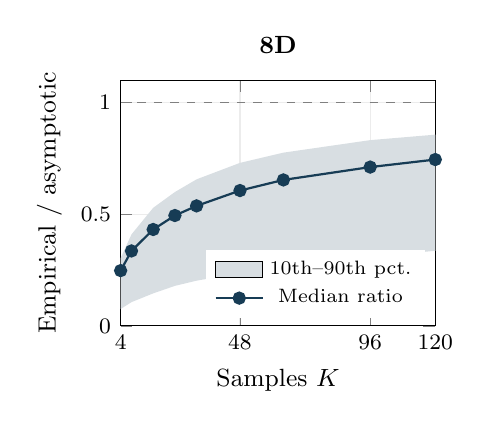
\begin{tikzpicture}
\begin{axis}[width=0.46\linewidth,height=4.7cm,xmin=4,xmax=120,xtick={4,48,96,120},xlabel={Samples $K$},grid=major,grid style={gray!15},tick label style={font=\footnotesize},label style={font=\small},title style={font=\small\bfseries},legend style={draw=none,font=\scriptsize,at={(0.98,0.98)},anchor=north east},title={8D},ymin=0,ymax=1.1,ylabel={Empirical / asymptotic},legend style={draw=none,font=\scriptsize,at={(0.97,0.03)},anchor=south east}]
\addplot[name path=lower,draw=none,forget plot] coordinates {(4,0.07574) (8,0.10641) (16,0.14573) (24,0.17931) (32,0.20268) (48,0.23632) (64,0.27068) (96,0.30743) (120,0.33666)};
\addplot[name path=upper,draw=none,forget plot] coordinates {(4,0.30404) (8,0.40995) (16,0.52914) (24,0.59973) (32,0.65669) (48,0.73043) (64,0.77624) (96,0.83228) (120,0.85686)};
\addplot[fill=ink!17,draw=none] fill between[of=lower and upper];\addlegendentry{10th--90th pct.}
\addplot[ink,thick,mark=*] coordinates {(4,0.24768) (8,0.33584) (16,0.43196) (24,0.49457) (32,0.53770) (48,0.60640) (64,0.65398) (96,0.71151) (120,0.74524)};\addlegendentry{Median ratio}
\addplot[gray,dashed,forget plot] coordinates {(4,1)(120,1)};
\end{axis}
\end{tikzpicture}
\captionof{figure}{Median empirical-to-asymptotic risk ratio and 10th--90th percentile band across observations, using reported full-run values at selected sample counts. The dashed line indicates exact calibration; bands are not confidence intervals.}\label{fig:cal}
\end{minipage}\end{center}
The discrepancy is observation-dependent. If every risk were a common multiple of $\tau_i^2/K$, the same optimal allocation would follow. But the exact SNIS error has a random normalizer:
\begin{equation}
 R_i(K)=\frac1d\E_{q_i}\left[\frac{\norm{\sum_{k=1}^{K} w_{ik}(z_{ik}-\mu_i)}^2}{(\sum_{k=1}^{K}w_{ik})^2}\right].
\end{equation}
The numerator and denominator are dependent; finite-sample bias and rare weight events can distort the asymptotic approximation. The measured risk ratios vary substantially between observations, although the asymptotic score retains ranking information ($\rho=0.842$ and $0.789$ at 48 draws). The correct finite-budget objective depends on marginal changes in risk, not ranking alone. In these experiments, the exact asymptotic oracle is outperformed by the learned predictor and by cheap rules; this is evidence against treating the asymptotic objective as the finite-sample optimum, not against the asymptotic theorem itself.

\textbf{Task dependence and teacher cost.} In the original confirmation, 512-draw teachers gave 75\% fewer teacher density evaluations than 2048-draw teachers (409,600 vs. 1,638,400 per dimension), with no observed loss in posterior-mean accuracy. Each teacher budget uses one fitted predictor, so neither a general ranking nor a wall-clock saving follows. The task-aware method increased log-evidence MAE by 1.23--2.46\% across the six original settings. On fresh datasets the increase was 2.42\% and 2.06\% in 4D/8D; the ESS-derived allocator improved log-evidence MAE by only 0.12\% and 0.09\%. Context-noise allocation increased evidence MAE by 8.29\% and 8.77\%. Thus a policy that reduces posterior-mean error need not improve log evidence; the evidence does not show that the tested ESS policy is generally optimal for log evidence. In particular the asymptotic log-evidence variance $(\E_q[(p/q)^2]-1)/K$ is not itself an absolute-error objective.


\section{VAE transfer and reference checks}\label{app:vae}
\subsection{VAE inference and independent reference checks}
The VAE defines a more realistic inference problem: $z\sim\N(0,I_d)$, $q_\phi(z\mid x)=\N(m_\phi(x),\operatorname{diag}(s_\phi^2(x)))$ and $p_\theta(x\mid z)=\N(g_\theta(z),\sigma_x^2 I)$ with $\sigma_x=0.15$. The $8\times8$ handwritten-digit images are from scikit-learn. The encoder and decoder are trained using the evidence lower bound \cite{kingma2014},
\begin{equation}
 \mathcal L_{\mathrm{ELBO}}=\E_{q_\phi}[\log p_\theta(x\mid z)]-\KL(q_\phi(z\mid x)\|p(z)).
\end{equation}
The frozen VAE defines the posterior; a separate regression model predicts the sampling difficulty, using pixel, encoder and reconstruction features. An initial three-seed 4D pilot was inconclusive. A 25-seed evaluation per dimension gave very small measured reductions (0.265\% and about 0.069\%). I then selected a temperature-scaled or defensive prior-mixture proposal using separate validation images:
\begin{equation}
 q_{T,\lambda}(z\mid x)=(1-\lambda)\N(z;m_\phi(x),T^2\operatorname{diag}(s_\phi^2(x)))+\lambda\N(z;0,I_d).
\end{equation}
Selection used median ESS fraction. For each dimension the follow-up used 25 trained VAEs, 104 previously unused test images, two groups of 52 with 2496 draws per group and 12 matched online repetitions. References pooled two independent 32,768-draw importance-sampling passes. The results below are measured against these approximate references.
\begin{center}\begin{minipage}{\linewidth}\centering\small
\begin{tabular}{@{}r rrr r r@{}}
\toprule
$d$ & Uniform MSE & Task MSE & Reduction & 95\% paired $t$ interval & Seeds lower\\
\midrule
4&0.014399&0.013689&4.93\%&$[-0.000900,-0.000521]$&25/25\\
8&0.106940&0.106029&0.85\%&$[-0.001583,-0.000239]$&17/25\\
\bottomrule
\end{tabular}
\captionof{table}{Selected-proposal task-aware versus uniform, using approximate IS references.}
\end{minipage}\end{center}
The reference ESS fraction was below 1\% for 17.8\% and 53.9\% of reference observations. A 4D audit found one draw carrying 83.17\% of normalized weight despite 131,072 samples; independent repeats produced another extreme-weight event. Let $\mu_{\rm ref}=\mu+\delta$, and let $\widehat\mu_T,\widehat\mu_U$ be the two estimates. Then the measured paired squared-error difference is
\begin{equation}
 \Delta_{\rm ref}=\norm{\widehat\mu_T-\mu}^2-\norm{\widehat\mu_U-\mu}^2-2(\widehat\mu_T-\widehat\mu_U)^\top\delta.
\end{equation}
The cross term can distort a small effect. I therefore used HMC \cite{neal2011} as an alternative reference, sampling from the posterior with potential $U(z)=\norm z^2/2+\norm{x-g_\theta(z)}^2/(2\sigma_x^2)$. On a fixed exploratory subset of eight 8D VAEs and twelve images, 93 of 96 cases passed basic diagnostics (rank-normalized $\widehat R<1.01$, bulk ESS $>400$, acceptable integration and acceptance checks \cite{vehtari2021}). Four chains used 1,000 warmup and 2,000 retained draws each. Original allocations were frozen; the subset was not reallocated.
\begin{center}\begin{minipage}{\linewidth}\centering\small
\begin{tabular}{@{}lrrrr@{}}
\toprule
Reference (matched subset)&Uniform&Task&Reduction&Sign-flip $p$\\
\midrule
HMC, all chains&0.123149&0.122539&0.495\%&0.6953\\
HMC, chains 1--2&0.122436&0.121907&0.432\%&0.7344\\
HMC, chains 3--4&0.123990&0.123300&0.557\%&0.6563\\
Original IS&0.122121&0.121679&0.362\%&0.7734\\
\bottomrule
\end{tabular}
\captionof{table}{Seed-level comparison on diagnostically passing cases, eight seeds. Chain groups are reference sensitivity checks, not independent allocation experiments.}
\end{minipage}\end{center}
The all-chain paired difference was $-0.000610$, 95\% interval $[-0.004387,0.003168]$, with five of eight seeds favoring the task allocator. The interval is wide relative to the observed effect; HMC does not establish a reliable improvement. Low ESS motivates proposal repair rather than simply allocating more draws, but 1\% is a diagnostic threshold, not a universal impossibility bound. Further work will prioritize tractable posterior references rather than more VAE reference forensics.

\section{Reproducibility and supporting experimental records}
The original synthetic studies use the Phase 2 notebook and its 512/1024/2048 teacher-budget trial and confirmation files. The 2026 synthetic oracle-and-risk follow-up notebook uses the same generator and 512-draw training procedure. The original confirmation seeds are 1001--1025 and the fresh seeds are 2001--2025. The full-run outputs are: \path{baseline_summary.csv}, \path{paired_comparisons.csv}, \path{oracle_summary.csv}, \path{finite_sample_risk_summary.csv}, and the per-observation risk CSV. The figures for the original studies reproduce numerical summaries from the earlier full runs; the risk figures use selected reported sample counts. The additional 2026 experiments are documented in Appendix~\ref{app:new}. No simulations were performed solely to prepare this document. The per-coordinate metric is already averaged across latent coordinates and is not divided by $d$ again.

The VAE study uses the separate confirmation, proposal-follow-up and reference-audit notebooks. The direct HMC comparison is recorded in \path{hmc_coverage_by_seed.csv} and \path{seed_level_hmc_comparisons.csv}. Its seeds are 27002, 27003, 27008, 27011, 27015, 27018, 27020, 27022; the image indices within the fixed follow-up set are 2, 19, 26, 34, 40, 44, 48, 65, 66, 71, 88, 90. The HMC reference is approximate and the tested subset does not constitute a new independent VAE training experiment. The bibliography combines the references in both supplied reports.

\section{Additional 2026 experimental studies}\label{app:new}
\subsection{Full finite-sample oracle and controlled heterogeneity}
The full study uses 25 test batches per regime and dimension, with 84 observations per batch, $B=4032$, 1,024 repetitions per optimization bank and 2,048 for independent evaluation, as specified by the full notebook. Eight development datasets per regime select the inexpensive baseline. The original context-dependent mixture is compared with fixed scale, noise-only, separation-only, mismatch-only and combined fixed-scale settings. In the controlled regimes, the separation of the component means and the mean offset of the proposal are varied independently where specified. The gain reported in Table~\ref{tab:fulloracle} is the primary gate statistic from the supplied full-run outputs, not the mean per-batch gain of the pooled AB policy; these summaries have different aggregation and/or optimization banks. None passes the 2\% gate.
\begin{center}\begin{minipage}{\linewidth}\centering\small
\begin{tabular}{@{}llrrrl@{}}\toprule
$d$ & Regime & Gain (\%) & 95\% CI & Better /25 & Frozen cheap rule\\\midrule
4 & Original & 0.3219 & [0.2633, 0.3770] & 24 & Context noise\\
4 & Fixed scale & -0.3058 & [-0.3374, -0.2742] & 0 & Uniform\\
4 & Noise only & 0.2434 & [0.1633, 0.3205] & 22 & Context noise\\
4 & Separation only & -0.0533 & [-0.0927, -0.0149] & 8 & Separation\\
4 & Mismatch only & 0.3289 & [0.2727, 0.3853] & 25 & Mismatch\\
4 & Combined fixed scale & 1.2168 & [1.0930, 1.3551] & 25 & Separation\\\midrule
8 & Original & 0.4784 & [0.4193, 0.5395] & 25 & Context noise\\
8 & Fixed scale & -0.2055 & [-0.2216, -0.1888] & 0 & Uniform\\
8 & Noise only & 0.1257 & [0.0801, 0.1722] & 21 & Context noise\\
8 & Separation only & -0.1931 & [-0.2215, -0.1637] & 0 & Separation\\
8 & Mismatch only & 0.5235 & [0.4791, 0.5666] & 25 & Mismatch\\
8 & Combined fixed scale & 1.2308 & [1.0510, 1.4170] & 25 & Separation\\\bottomrule
\end{tabular}\captionof{table}{Primary full-study gate results supplied from the controlled oracle run. Intervals are paired across independent test batches.}\label{tab:fulloracle}\end{minipage}\end{center}
Compared with fixed scale, combined heterogeneity increased measured headroom by 1.523 and 1.436 percentage points (4D and 8D); mismatch alone increased it by 0.635 and 0.729 points. Because the frozen cheap rule differs across regimes, these contrasts are not pure causal interactions. The mean fitted risk-decay exponents range from 0.714 to 0.846, below the inverse-$K$ exponent of one. In 4D fixed scale, bank A indicated a training gain of 0.775\%, but independent evaluation yielded a loss of about 0.306\%. Such optimism illustrates optimization over noisy Monte Carlo curves. The pooled bank reduced the observed loss without establishing positive headroom.
\subsection{Real-data inference model and split}
The UJIIndoorLoc data contain 19,937 official development and 1,111 official held-out records, with 520 wireless access points. From user-disjoint development groups, the final run uses 11,803 fit observations, 1,600 calibration observations, 1,000 risk-teacher observations and 512 validation observations (capped on development data). The map comprises 779 discrete states, defined by surveyed building, floor and rounded coordinates. The likelihood combines independent Bernoulli detection indicators and conditional Gaussian signal strengths, smoothed toward floor and global statistics. Let $D_a$ indicate access point detection and $r_a$ be the standardized signal when detected. The likelihood has the form
\begin{equation}
 L(x\mid s)=\prod_{a=1}^{520} \eta_{sa}^{D_a}(1-\eta_{sa})^{1-D_a}\left[\mathcal N(r_a;m_{sa},v_{sa})\right]^{D_a}.
\end{equation}
The fitted model uses a calibrated temperature on the state scores; its normalized posterior is evaluated by finite summation for offline labels and references. A neural proposal learned on development records uses a defensive uniform component to preserve support. The partition contains 32 fixed regions obtained by clustering survey coordinates within building-floor groups. The posterior student learns a distribution over all 779 states from soft target labels on fit records; region masses and conditional moments follow from sums of its predicted probabilities. Student temperature is selected on the calibration group. At allocation time the student, the neural proposal, the map and observed signals are accessible, but exact posterior scores are not supplied to the learned allocator. The code explicitly checks that removing target labels does not change its online features.

The reference is exact for this fitted discrete model, not a claim that the model is the physical ground truth. The primary metric is per-coordinate squared error relative to the model posterior mean; Euclidean coordinate errors relative to recorded locations are reported separately. The test records are reused across all three real-data runs, with different Monte Carlo seeds and settings. The real-data confidence intervals quantify Monte Carlo uncertainty conditional on the fixed records, not uncertainty across new users, buildings or deployments.
\subsection{Exploratory progression on the real-data pipeline}
\begin{center}\begin{minipage}{\linewidth}\centering\small
\begin{tabularx}{\linewidth}{@{}Yrrr@{}}\toprule
Policy (gain vs. cheap, \%) & Initial & Coverage & Structured\\\midrule
Estimated finite-sample oracle & 30.54 & 28.72 & 31.67\\
Privileged coverage & -- & 24.84 & 26.03\\
Privileged inverse-$K$ & -- & 12.92 & 4.10\\
Learned policy under study & -19.55 & -29.66 & 8.20\\
\bottomrule\end{tabularx}\captionof{table}{Within-run gains relative to floor-uncertainty allocation. Runs use different training, Monte Carlo banks and batch compositions; these are not paired cross-run comparisons.}\end{minipage}\end{center}
The initial generic power-law predictor failed; validation selected full fallback ($\alpha=0$). The coverage study gave a 13.69\% MSE reduction for privileged coverage relative to privileged inverse-$K$, capturing 86.49\% of estimated oracle headroom. The learned direct-coefficient variant was unsuccessful. The final structured study reconstructs the coefficient from posterior moments and masses instead of predicting it directly. In the final run, the learned risk comparators receive matched student-derived features; every policy obeys $4\le K_i\le120$ and exactly $48n$ draws per batch. In the real-data study, 35 batches of at most 32 observations consume 53,328 draws per replicate in total. The final run uses 512 teacher repetitions, 512 per oracle bank and 1,024 for independent evaluation. The final run was on CPU. The manifest records 30 epochs; the full notebook separately configures 50 epochs for the structured student. The manifest does not independently record the completed student epoch count.
\begin{center}\begin{minipage}{\linewidth}\centering\small
\begin{tabular}{@{}lrr@{}}\toprule
Comparator & Structured MSE reduction (\%) & Conditional 95\% CI\\\midrule
Inexpensive rule & 8.1956 & [7.4915, 8.8997]\\
Matched-feature generic learner & 0.4695 & [-0.2040, 1.1430]\\
Learned inverse-$K$ & 22.1444 & [21.0642, 23.2246]\\
Direct coefficient learner & 31.1901 & [30.2095, 32.1708]\\\bottomrule
\end{tabular}\captionof{table}{Final run's primary paired contrasts, conditional on the reused real test records. The comparison with the generic learner is inconclusive.}\end{minipage}\end{center}
\begin{center}\begin{minipage}{\linewidth}\centering\small
\begin{tabular}{@{}lrr@{}}\toprule
Component substitution & MSE & Gain vs. structured (\%)\\\midrule
Fully learned structured & 49.9309 & 0.00\\
Exact mass, predicted moments & 59.7187 & -19.60\\
Predicted mass, exact moments & 49.9835 & -0.11\\
Exact mass and moments & 59.9621 & -20.09\\\bottomrule
\end{tabular}\captionof{table}{Privileged diagnostic substitutions with the fitted amplitude and validation parameters held fixed. They do not represent separately retrained predictors.}\end{minipage}\end{center}
The final student's region-mass mean absolute error is 0.0119. Spearman correlations for predicted region sensitivity, coverage at 48 and coverage marginal reduction over 24--72 are 0.1923, 0.5986 and 0.7565, respectively. The high marginal correlation does not guarantee optimal allocation. Structured allocation is worse than the cheap policy in 40\% of batches; the generic learner harms 31.43\%. The final all-criteria gate is not passed, despite meeting the point gain and 25\% headroom targets. The estimated oracle headroom captured is $(54.3883-49.9309)/(54.3883-37.1642)=25.88\%$ using unrounded values in computation.
\begin{center}\begin{minipage}{\linewidth}\centering\small
\begin{tabular}{@{}lrr@{}}\toprule
Method & Mean coordinate error & Median latency (ms)\\\midrule
Exact discrete posterior & 8.666 & 1.82\\
Direct posterior student & 16.782 & 2.64\\
Uniform SNIS & 10.118 & 14.67\\
Inexpensive allocation & 9.868 & 20.08\\
Structured coverage & 9.804 & 77.14\\
Generic learner & 9.794 & 90.55\\\bottomrule
\end{tabular}\captionof{table}{Final run: mean physical-coordinate error in native coordinate units (metres not independently verified), and median of 15 CPU timings on one batch. This benchmark does not establish a general speed advantage.}\end{minipage}\end{center}
\subsection{Earlier synthetic coverage study}
Before structured posterior reconstruction, the coverage method regressed region sensitivity coefficients directly. This exploratory run used 12 fresh synthetic test batches per setting, 384 teacher repetitions, two 256-repetition optimization banks and 512 independent evaluation repetitions. The learned coverage gain was below the 2\% target in all six configurations. The earlier real-data run's validation-selected coverage coefficient was $\gamma=0.25$ and full shrinkage selected $\alpha=0$. The following table preserves the earlier synthetic results; the final study uses different cohorts and need not reproduce these point estimates.
\begin{center}\begin{minipage}{\linewidth}\centering\small
\begin{tabular}{@{}llrr@{}}\toprule
$d$ & Regime & Gain vs. cheap (\%) & Gain vs. generic (\%)\\\midrule
4 & Original & 0.6470 & -0.0694\\
4 & Separation & -0.0131 & 0.0001\\
4 & Mismatch & 0.2040 & -0.0134\\
8 & Original & 0.2510 & -0.2216\\
8 & Separation & 0.0884 & -0.0068\\
8 & Mismatch & 0.1704 & 0.0048\\\bottomrule
\end{tabular}\captionof{table}{Exploratory direct-coefficient coverage study. Gains refer to unshrunk coverage allocations and are not evidence of a practically meaningful improvement.}\end{minipage}\end{center}
\clearpage
\subsection{Final fresh synthetic confirmation}
The final notebook evaluates six synthetic cases using 25 independent 84-observation test batches per case, distinct from its distillation, teacher and validation cohorts. The synthetic partition consists of 15 rectangles in the first two coordinates with remaining axes unrestricted. Analytic Gaussian interval masses and first moments provide offline labels. The student is trained on 4,032 development observations, with 1,008 risk-teacher and 504 validation observations per case. The 2\% criterion is not met in any case. Holm correction is applied to the primary cheap and generic comparisons across the six synthetic cases.
\begin{center}\begin{minipage}{\linewidth}\centering\small
\begin{tabular}{@{}llrrr@{}}\toprule
$d$ & Regime & Gain vs. cheap (\%) & 95\% CI & Gain vs. generic (\%)\\\midrule
4 & Original & 0.6722 & [0.6071, 0.7373] & -0.0357\\
4 & Separation & -0.0192 & [-0.0509, 0.0126] & -0.0730\\
4 & Mismatch & 0.2312 & [0.1911, 0.2712] & -0.0041\\
4 & Combined & 0.1290 & [0.0865, 0.1716] & -0.0521\\
8 & Original & 0.2165 & [0.1647, 0.2683] & -0.2817\\
8 & Combined & 0.2090 & [0.1841, 0.2339] & -0.0512\\\bottomrule
\end{tabular}\captionof{table}{Fresh synthetic results from the final structured study. The small gains are consistent with the earlier low-headroom study; no case passes the full gate.}\end{minipage}\end{center}
\subsection{Additional reproducibility records}
The full oracle table and heterogeneity contrasts were supplied as notebook output tables and plots. The other three new studies are recorded in the notebooks \path{UJIIndoorLoc_Finite_Sample_Risk_Real_Application.ipynb}, \path{Coverage_Aware_SNIS_Allocation.ipynb}, and \path{Final_Structured_Coverage_SNIS_Allocation.ipynb}, with the corresponding results archives. The full controlled study uses \path{Finite_Sample_Oracle_and_Controlled_Heterogeneity.ipynb}. The final archive contains the manifest, \path{final_gate_summary.csv}, \path{all_primary_contrasts.csv}, \path{wifi/method_summary.csv}, \path{wifi/component_ablations.csv}, \path{wifi/runtime_summary.csv}, \path{wifi/region_diagnostics.json}, per-case allocation counts, validation selections and fitted models. The dataset checksum recorded by all three real-data runs is \texttt{893512b82dfd7a7c345d84195b1c8019fbca0fa0d7820ce491ce5aa45ec3782f}. Final manifest seed: 20261123; new seed: 932011. The new summaries reproduce exported results; no experiment is rerun in preparing the proposal.
\clearpage
\begin{thebibliography}{99}
\bibitem{owen2013} A. B. Owen. \emph{Monte Carlo Theory, Methods and Examples}. 2013. \url{https://artowen.su.domains/mc/}.
\bibitem{kingma2014} D. P. Kingma and M. Welling. Auto-encoding variational Bayes. \emph{International Conference on Learning Representations}, 2014. \url{https://arxiv.org/abs/1312.6114}.
\bibitem{burda2016} Y. Burda, R. Grosse, and R. Salakhutdinov. Importance weighted autoencoders. \emph{International Conference on Learning Representations}, 2016. \url{https://arxiv.org/abs/1509.00519}.
\bibitem{rainforth2018} T. Rainforth et al. Tighter variational bounds are not necessarily better. \emph{Proceedings of the 35th International Conference on Machine Learning}, 2018. \url{https://proceedings.mlr.press/v80/rainforth18b.html}.
\bibitem{tucker2019} G. Tucker, D. Lawson, S. Gu, and C. J. Maddison. Doubly reparameterized gradient estimators for Monte Carlo objectives. \emph{International Conference on Learning Representations}, 2019. \url{https://arxiv.org/abs/1810.04152}.
\bibitem{neal2011} R. M. Neal. MCMC using Hamiltonian dynamics. In \emph{Handbook of Markov Chain Monte Carlo}, Chapman and Hall/CRC, 2011. \url{https://arxiv.org/abs/1206.1901}.
\bibitem{vehtari2021} A. Vehtari, A. Gelman, D. Simpson, B. Carpenter, and P.-C. B\"urkner. Rank-normalization, folding, and localization: An improved $\widehat R$ for assessing convergence of MCMC. \emph{Bayesian Analysis}, 16(2):667--718, 2021. \url{https://doi.org/10.1214/20-BA1221}.

\bibitem{neyman1934} J. Neyman. On the two different aspects of the representative method: the method of stratified sampling and the method of purposive selection. \emph{Journal of the Royal Statistical Society}, 97(4):558--625, 1934.
\bibitem{chatterjee2018} S. Chatterjee and P. Diaconis. The sample size required in importance sampling. \emph{Annals of Applied Probability}, 28(2):1099--1135, 2018.
\bibitem{martino2017} L. Martino, V. Elvira, and F. Louzada. Effective sample size for importance sampling based on discrepancy measures. \emph{Signal Processing}, 131:386--401, 2017.
\bibitem{bugallo2017} M. F. Bugallo, V. Elvira, L. Martino, D. Luengo, J. M\'iguez, and P. M. Djuri\'c. Adaptive importance sampling: the past, the present, and the future. \emph{IEEE Signal Processing Magazine}, 34(4):60--79, 2017.
\bibitem{gershman2014} S. Gershman and N. Goodman. Amortized inference in probabilistic reasoning. \emph{Proceedings of the Annual Meeting of the Cognitive Science Society}, 36, 2014.
\bibitem{cremer2018} C. Cremer, X. Li, and D. Duvenaud. Inference suboptimality in variational autoencoders. ICML, 2018.
\bibitem{cranmer2020} K. Cranmer, J. Brehmer, and G. Louppe. The frontier of simulation-based inference. \emph{PNAS}, 117(48):30055--30062, 2020.
\bibitem{uji2014} J. Torres-Sospedra et al. UJIIndoorLoc [Dataset]. UCI Machine Learning Repository, 2014. \url{https://doi.org/10.24432/C5MS59}.
\end{thebibliography}
\end{document}
